\chapter{Objetivos}
\label{cap:capitulo2}

En esta sección del documento se describe el problema a resolver, marcando los objetivos y requisitos pautados en el desarrollo del \ac{TFG}.

\section{Descripción del problema}
\label{sec:descripcion}

El objetivo principal de este \ac{TFG} es desarrollar un sistema de conducción autónoma capaz de desenvolverse eficientemente en entornos urbanos. Para lograrlo, se emplean técnicas de \ac{DRL} para la toma de decisiones, junto con diferentes enfoques de \ac{DL} para la percepción del entorno, con el objetivo de garantizar un comportamiento robusto, seguro y eficiente. El proyecto se centra en conseguir una conducción segura y estable durante todo el recorrido, abordando tres subtareas principales: seguimiento del carril, control adaptivo respecto al vehículo de delante y llevar a cabo una maniobra de adelantamiento completa.

A continuación, se definen los siguientes sub-objetivos: 

\begin{enumerate}
\item Desarrollo de un comportamiento de sigue-carril basado en \ac{DL} para la percepción y en algoritmos de \ac{DRL} para la toma de decisiones.
\item Ampliación del comportamiento de seguimiento de carril para incorporar una respuesta adaptativa al tráfico, manteniendo una velocidad de crucero ajustada al vehículo que circula delante del coche autónomo.
\item Desarrollo de un modelo basado en \ac{DRL} capaz de ejecutar maniobras completas de adelantamiento, incluyendo el cambio de carril y la vuelta al mismo.
\item Análisis y comparación de los diferentes comportamientos de conducción autónomos desarrollados.
\end{enumerate}

\section{Requisitos}
\label{sec:requisitos}

Los requisitos que han de cumplirse en este trabajo son:
\begin{enumerate}
\item Uso del entorno de simulación CARLA\footnote{\url{https://carla.org/}}, el cual permite la simulación de escenarios realistas, diversos comportamientos de vehículos y la prueba de modelos. Al ser un simulador ampliamente reconocido en el ámbito de la conducción autónoma, garantiza la reutilización del proyecto en aplicaciones futuras de este campo.
\item Lograr un comportamiento de sigue-carril estable y sin oscilaciones, alcanzando velocidades en torno a los 70 km/h.
\item Mantener el control adaptativo al tráfico asegurando una distancia de seguridad adecuada respecto al vehículo delantero, de acuerdo con las normas de la \ac{DGT}\footnote{\url{https://www.dgt.es/export/sites/web-DGT/.galleries/downloads/conoce-el-estado-del-trafico/operaciones-especiales/4_O.-E.-Primero-de-Mayo-2023_Consejos-y-normas-de-Seguridad-Vial_V-I.pdf}}.
\end{enumerate}

\section{Metodología}
\label{sec:metodologia}

Este TFG comenzó en febrero de 2024 y finalizó en marzo de 2025. La metodología de trabajo fue la siguiente:

\begin{itemize}
\item Se siguió la metodología \textit{Scrum}\footnote{\url{https://www.nimblework.com/agile/scrum-methodology/}}, utilizada para la gestión de proyectos organizando el trabajo en ciclos cortos llamados \textit{sprints}, que suelen durar de una y cuatro semanas. Esta metodología fomenta una organización eficiente al dividir el trabajo en tareas pequeñas y manejables, promoviendo la iteración y mejora continua al revisar y ajustar el trabajo regularmente.
\item Durante cada \textit{sprint}, se realizaron reuniones semanales a través de \textit{Teams}\footnote{\url{https://www.microsoft.com/es-es/microsoft-teams/log-in}}, con una duración de entre 30 y 60 minutos, para hacer un seguimiento de los problemas que hubieran podido surgir durante la semana y definir los nuevos objetivos a cumplir.
\item Contacto mediante el email de la universidad con el fin de resolver problemas urgentes e intercambiar contenido de avances significativos logrados.
\item Se utilizó un repositorio de \textit{GitHub}\footnote{\url{https://github.com/}} para gestionar el control de versiones del código fuente, los modelos y los datos más relevantes generados durante el desarrollo del proyecto. En la Figura \ref{fig:github}, se observa que la mayor carga de trabajo tuvo lugar al inicio, coincidiendo con la creación de los entornos de desarrollo y la implementación de los módulos de percepción. Posteriormente, se llevaron a cabo los entrenamientos y pruebas de los modelos, ajustando los hiperparámetros de entrenamiento e intentando mejorar los resultados obtenidos. Finalmente, se ve un último \textit{sprint} referente a la elaboración memoria y a los ajustes finales en los entrenamientos del adelantamiento.

\begin{figure}[ht]
\centering
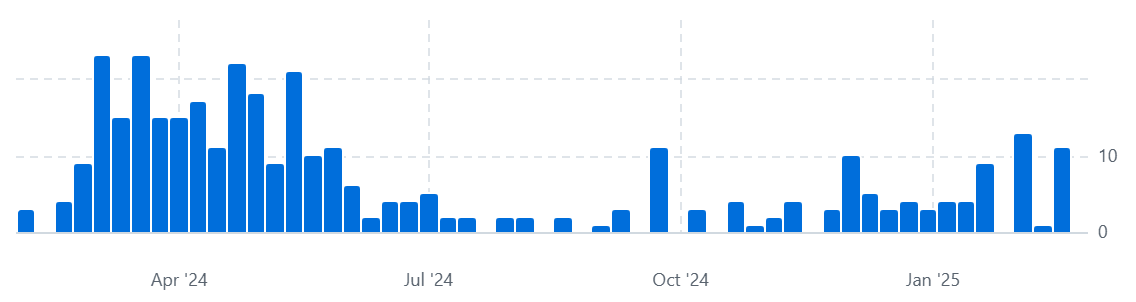
\includegraphics[width=7cm]{figs/objetivos/github.png}
\caption{Seguimiento de trabajo en GitHub.}
\label{fig:github}
\end{figure}

\item Mantenimiento de un \textit{blog}\footnote{\url{https://roboticslaburjc.github.io/2024-tfg-lara-poves/}} con el propósito de documentar problemas, avances e investigaciones realizadas durante el desarrollo del proyecto, asegurando un registro del progreso y soluciones de los desafíosplateados.

\end{itemize}

\section{Plan de trabajo}
\label{sec:plantrabajo}

Finalmente, los pasos a seguir fueron:

\begin{enumerate}
\item Comienzo del trabajo:
\begin{itemize}
\item Desde el inicio, el tema del proyecto estuvo claro, centrado en la conducción autónoma en el simulador CARLA y algoritmos de \ac{DRL}.
\item Se gestionó el acceso al servidor donde se desarrollaría el proyecto, el cual ya contaba con el simulador CARLA instalado. 
\item Se creó un entorno \textit{Conda}\footnote{\url{https://anaconda.org/}} y se procedió a la instalación de las librerías necesarias para el desarrollo del proyecto.
\end{itemize}

\item Desarrollo del proyecto:
\begin{itemize}
\item Se desarrolló un teleoperador sencillo para explorar las diversas funcionalidades y configuraciones que ofrece el simulador CARLA.
\item Se implementó el manejo y visualización de los sensores, \ac{LiDAR} y la cámara RGB, cuyos datos se utilizarán posteriormente para lograr los comportamientos autónomos fijados. Además, se integraron redes neuronales para la detección del carril y la segmentación semántica de la calzada. Para la identificación del carril, también se incluyó una nueva forma de detección basada en \textit{ground truth} en CARLA. 
\item Se configuró el autopiloto de CARLA, explorando las distintas opciones de configuración disponibles.
\item A partir de los datos de los sensores y las herramientas integradas, se implementó la detección del carril, calculando variables como su área y centro de masas. Además, se aplicó un tratamiento inteligente a la nube de puntos del \ac{LiDAR}, filtrando estos puntos para detectar otros vehículos en la carretera.
\item Se desarrolló un sistema de seguimiento de carril basado en un controlador \ac{PID}.
\item En una primera etapa, se entrenó un modelo utilizando \ac{DQN} para que fuera capaz de seguir el carril. Posteriormente, se entrenó un nuevo modelo utilizando \ac{PPO} para mejorar el desempeño.
\item Se realizó un reentrenamiento del último modelo para lograr mantener una velocidad de crucero respecto al vehículo delantero utilizando la información proporcionada por el \ac{LiDAR}.
\item Finalmente, se entrenó un nuevo modelo para conseguir realizar una maniobra de adelantamiento completa en un entorno controlado.
\end{itemize}

\item Evaluación: Se compararon y analizaron los resultados obtenidos durante las diferentes fases y modelos del proyecto.
\item Se redactó la memoria del trabajo, documentando todo el proceso de investigación y desarrollo realizado.
\end{enumerate}

